\chapter{Appendix of ``Love the Candidate but Hate his Party: The Asymmetric Effects of Reelection Incentives on Partisan and Personal Incumbency Returns in Mexico'' \label{chap:append2}}

\break

%\section{Tables and Figures}

\begin{table}[H]
\centering 
\caption{Descriptive statistics}
   
\label{tab:descriptive}
\scalebox{0.55}{ 
{
\def\sym#1{\ifmmode^{#1}\else\(^{#1}\)\fi}
\begin{tabular}{l*{1}{ccccc}}
\hline\hline
            &        \textbf{Mean}&  \textbf{SD}&  \textbf{Min}&  \textbf{Max}& \textbf{N}\\
\hline    
\emph{Pane A - Incumbency Advantage:} 	&		&		&		&		\\
Probability of winning, election at t+1&        0.40&        0.49&           0&           1&       2,247\\
Vote share, election at t+1&       -0.05&        0.18&          -1&         .59&       2,246\\

\\
\emph{Panel B - Treatments and Forcing Variable:} 	&		&		&		&		\\
Term Limit Removed=1; 0 otherwise&        0.29&        0.45&           0&           1&       2,247\\
Win election at t=1; 0 otherwise&        0.46&        0.50&           0&           1&       2,247\\

Winning margin: first - second runner&        0.07&        0.05&        0.00&        0.33&       2,247\\


\\
\emph{Panel C - Pretreatment controls:} 	&		&		&		&		\\
Winning margin: first - second runner (governor)&        0.15&        0.13&           0&           1&      24,470\\
Party alignment with federal executive=1; 0 otherwise&        0.54&        0.50&           0&           1&      24,470\\

Population (INEGI and CONAPO projections)&      49,233&     129,415&         409&   1,714,709&       2,247\\


\\
\emph{Panel D - Mechanisms-Fiscal Transfers:} 	&		&		&		&		\\
General Participations Fund (Mill. pesos)&          39&          94&         .81&       1,221&       1,638\\
Participating Fund (Mill. pesos)&          52&         127&         .21&       1,498&       1,656\\
Municipal Development Fund (Mill. pesos)&         9.7&          24&          .2&         345&       1,642\\
Federal and state contributions (Mill. pesos)&          60&         131&        .048&       2,133&       1,768\\
Contribution Fund for Municipal Social Infrastructure (Mill. pesos)&          18&          30&        .048&         618&       1,759\\
Contribution Fund to Strengthen Municipalities (Mill. pesos)&          23&          61&         .15&         865&       1,755\\

\\
\emph{Panel E - Mechanisms-Municipal Revenues:} 	&		&		&		&		\\
Total Municipal Revenues (Mill. pesos)&         166&         420&           2&       5,715&       1,779\\
Tax Revenues (Mill. pesos)&          19&          82&      .00017&       1,256&       1,735\\
Property Tax Rrevenues (Mill. pesos)&          12&          48&      .00013&         476&       1,360\\
Estate Tax Revenues (Mill. pesos)&          17&          66&      .00013&         672&       1,506\\
Prod., Cons. and Trans. Tax Revenues (Mill. pesos)&         1.2&          19&     .000096&         488&         671\\
Vehicle Ownership Tax Revenues (Mill. pesos)&          .5&         1.9&     .000081&          29&       1,324\\
New Cars Tax Revenues (Mill. pesos)&         .87&         2.9&       .0032&          49&       1,530\\
Public Security Revenues (Mill. pesos)&         6.1&          15&     .000078&         121&         211\\

\\
\emph{Panel F - Mechanisms-Other Resources:} 	&		&		&		&		\\
Number of City Council Sessions&          23&          19&           0&         288&       1,784\\
Number of Approved Initiatives of Law&          17&          32&           0&         295&         884\\
Percentage of Municipal Budget Spend&          11&          15&           0&         100&         789\\
Bureaucrats per 100,000 inhabitants&       1,945&       2,601&           0&      24,528&       1,247\\

\\
\emph{Panel G - Mechanisms-Incumbents' quality:} 	&		&		&		&		\\
Incumbent undergraduate or graduate title (indicator)&        0.06&        0.24&           0&           1&      19,430\\

\\ 

\hline\hline
\end{tabular}    
}
}
\end{table} 
   


 \begin{figure}[h]   
\centering
 \caption{No discontinuous jump of covariates}
 \label{fig:jump_covariates}
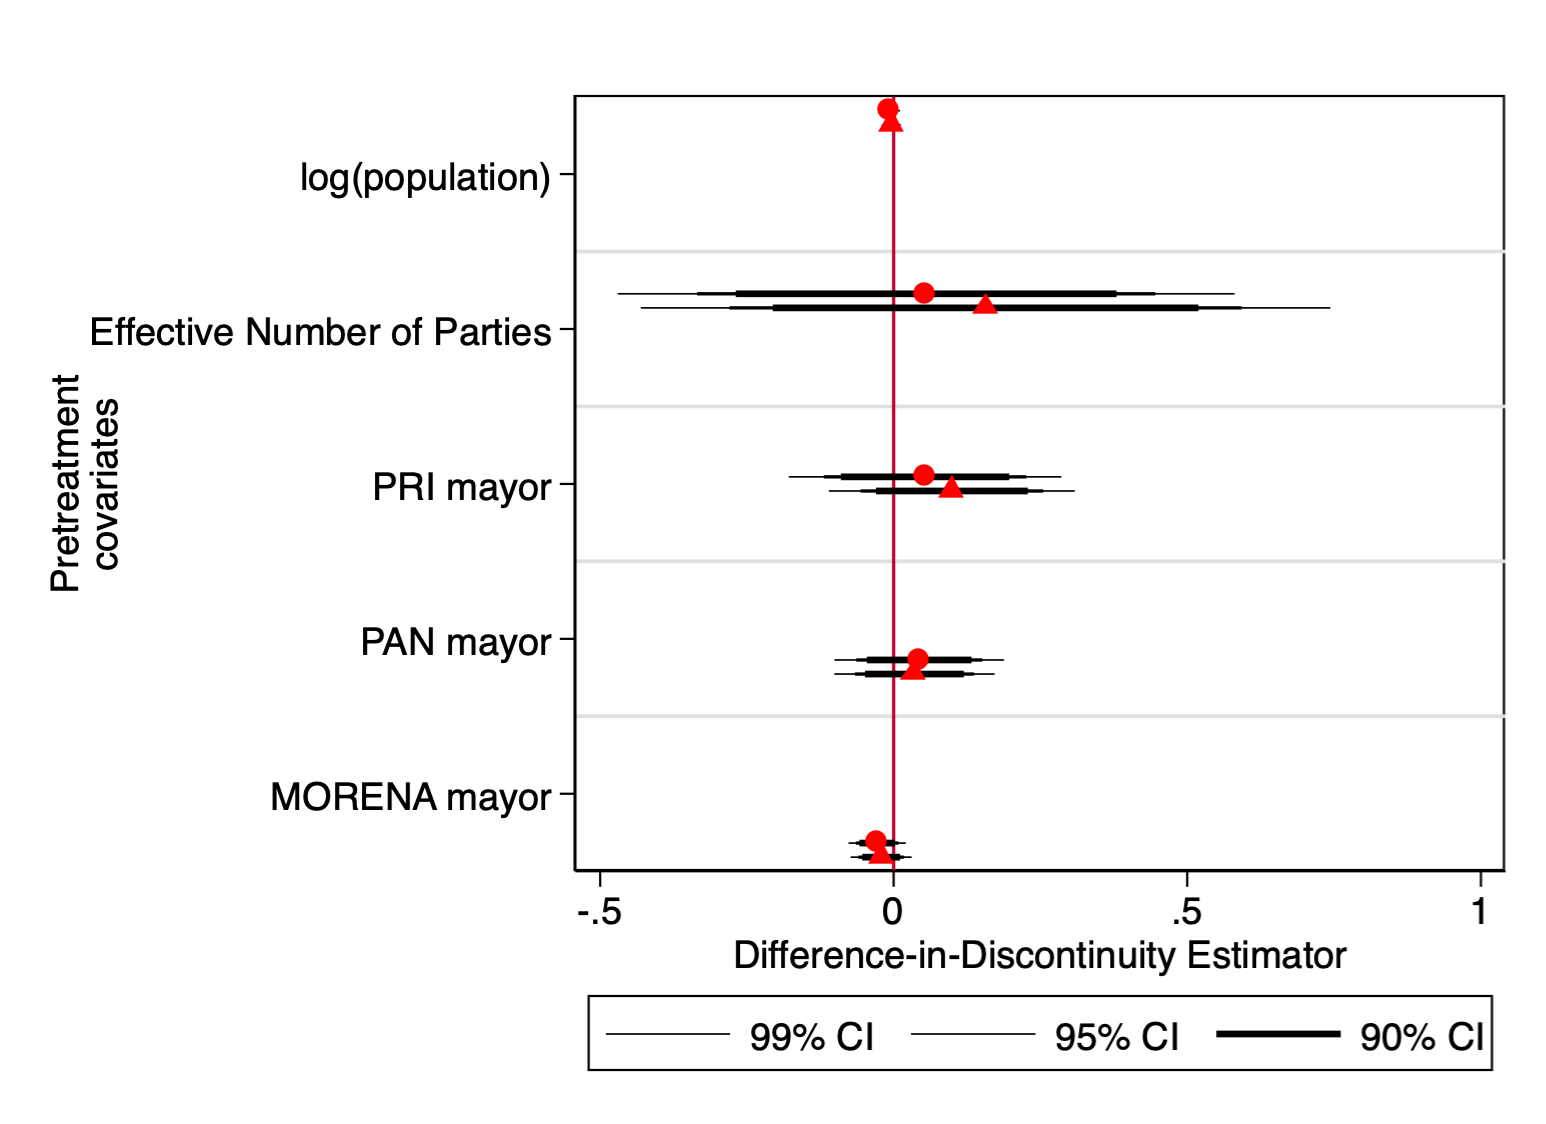
\includegraphics[width=0.9\textwidth]{Chapter2/Figures_incumbency/nojump.png}
       \captionsetup{justification=centering}
    
 \textbf{Note:} Figure \ref{fig:jump_covariates} shows the average treatment effect of the Term Limit Reform on various pretreatment covariates using a difference in discontinuity of close elections design. Optimal bandwidths following \citet{calonicoetal_2014} are used. 
   
\end{figure} 

  
    
    
\begin{figure}[h]   
\centering
 \caption{McCrary Test}
 \label{fig:mccrary}
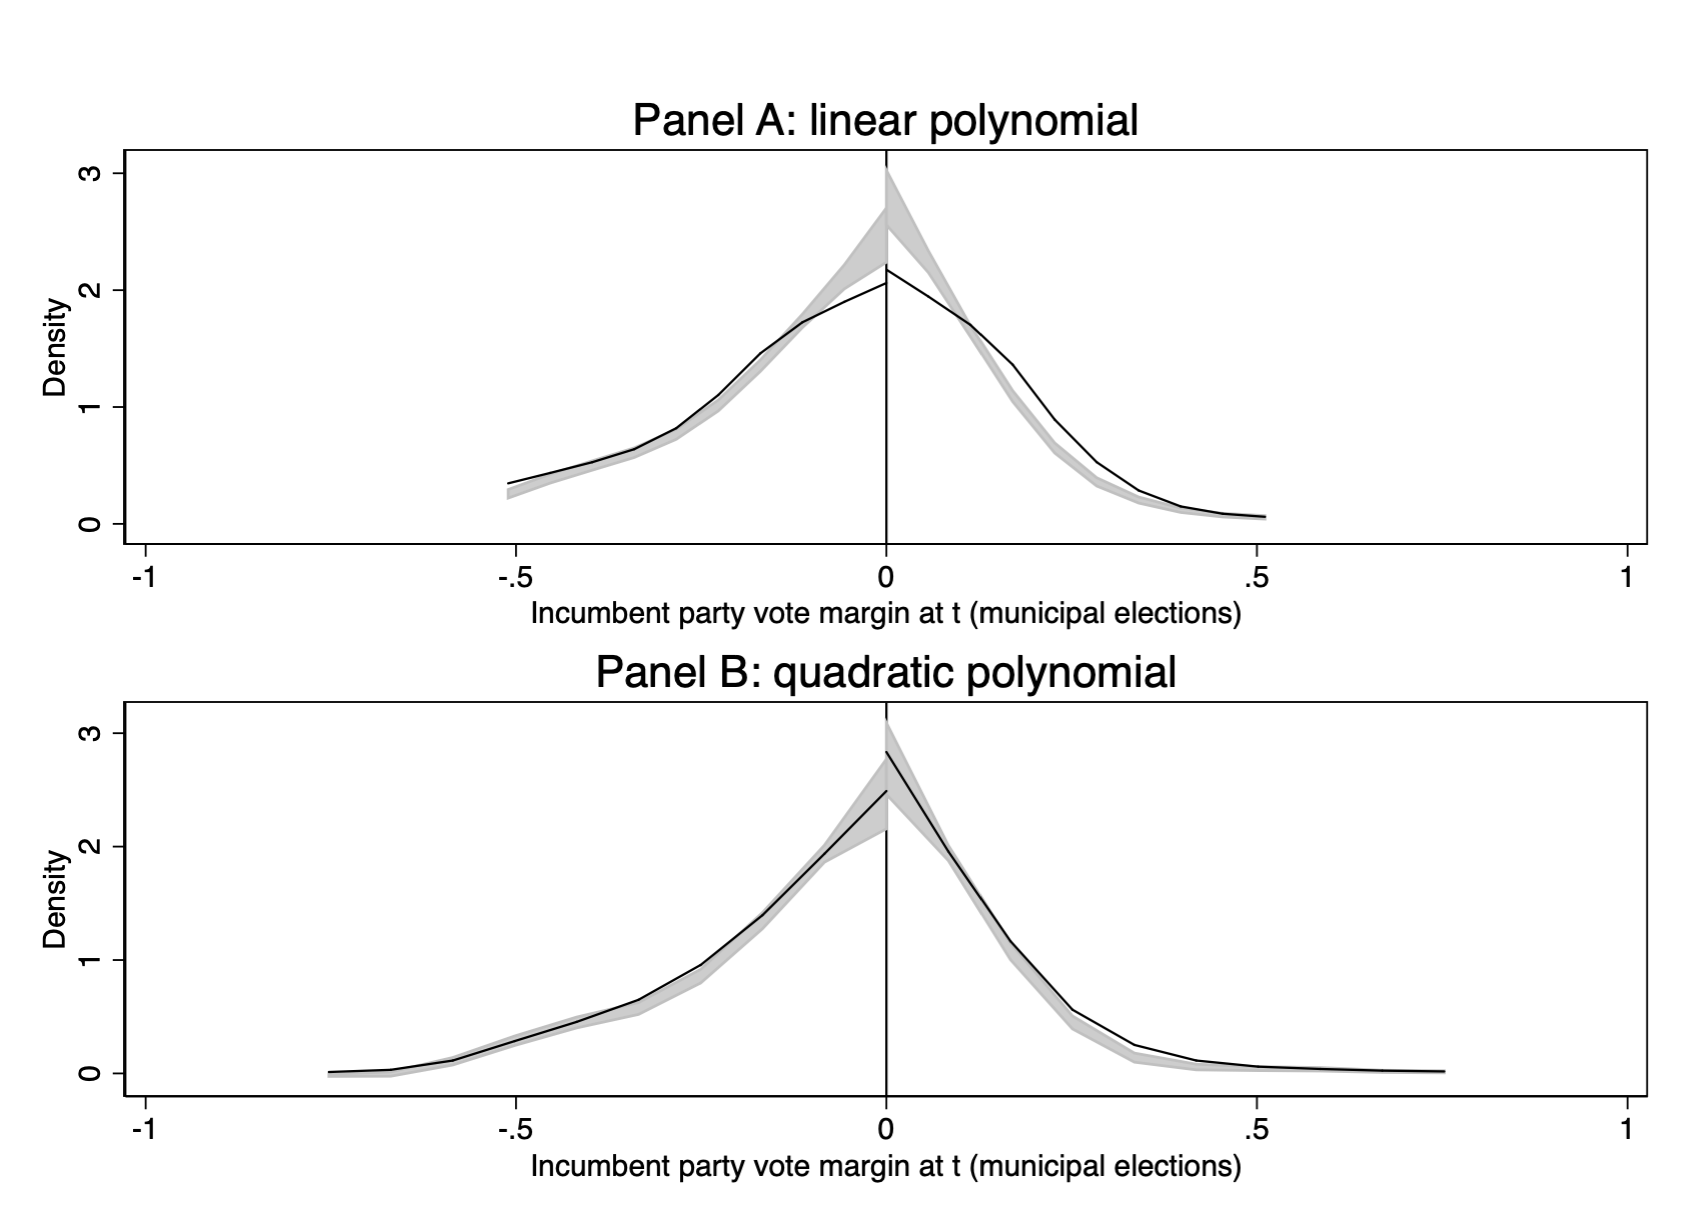
\includegraphics[width=1\textwidth]{Chapter2/Figures_incumbency/mccrary_pol1_2.png}
%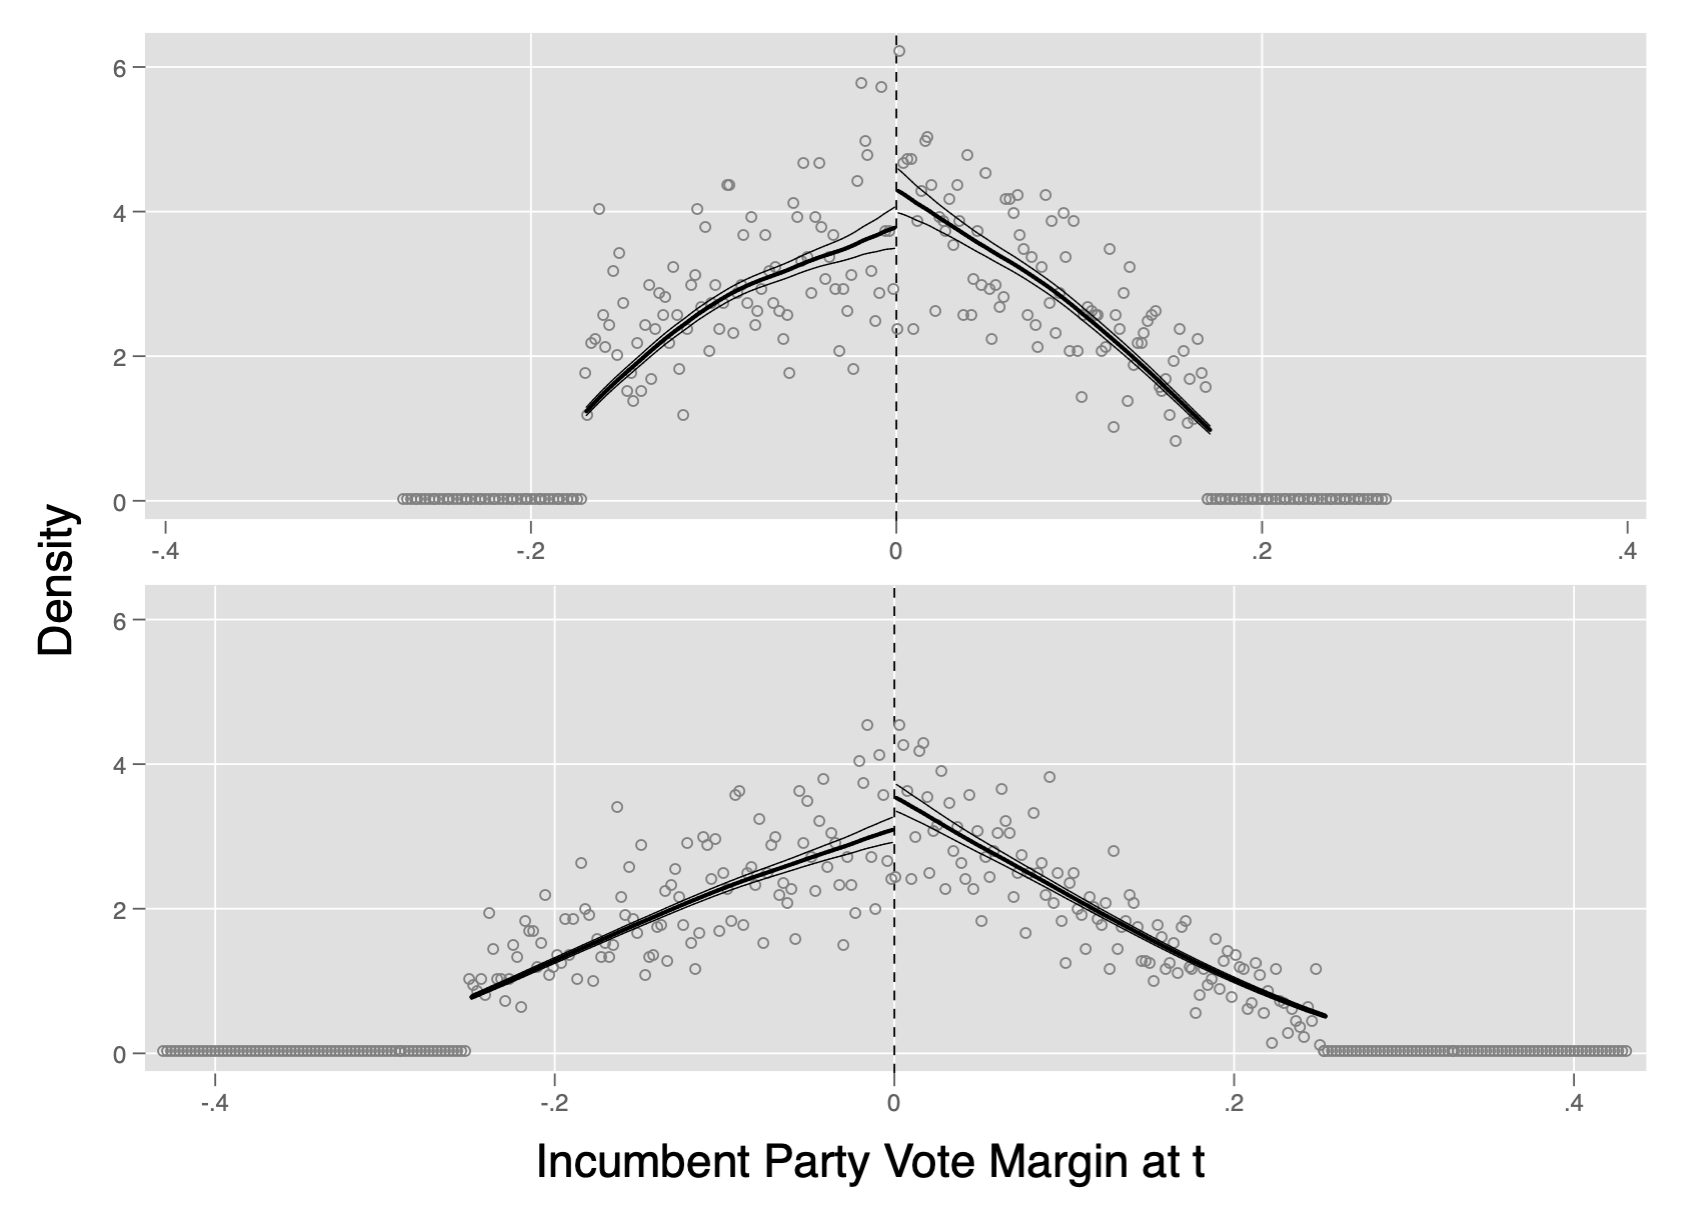
\includegraphics[width=0.9\textwidth]{../Figures/conditional_mccrary_test_pol1_final.png}

       \captionsetup{justification=centering}
         
 \textbf{Note:} 95\% confidence intervals reported.
 
\end{figure} 


 \begin{figure}[h]   
\centering
 \caption{Testing Different Bandwidths}
 \label{fig:bandwidths}
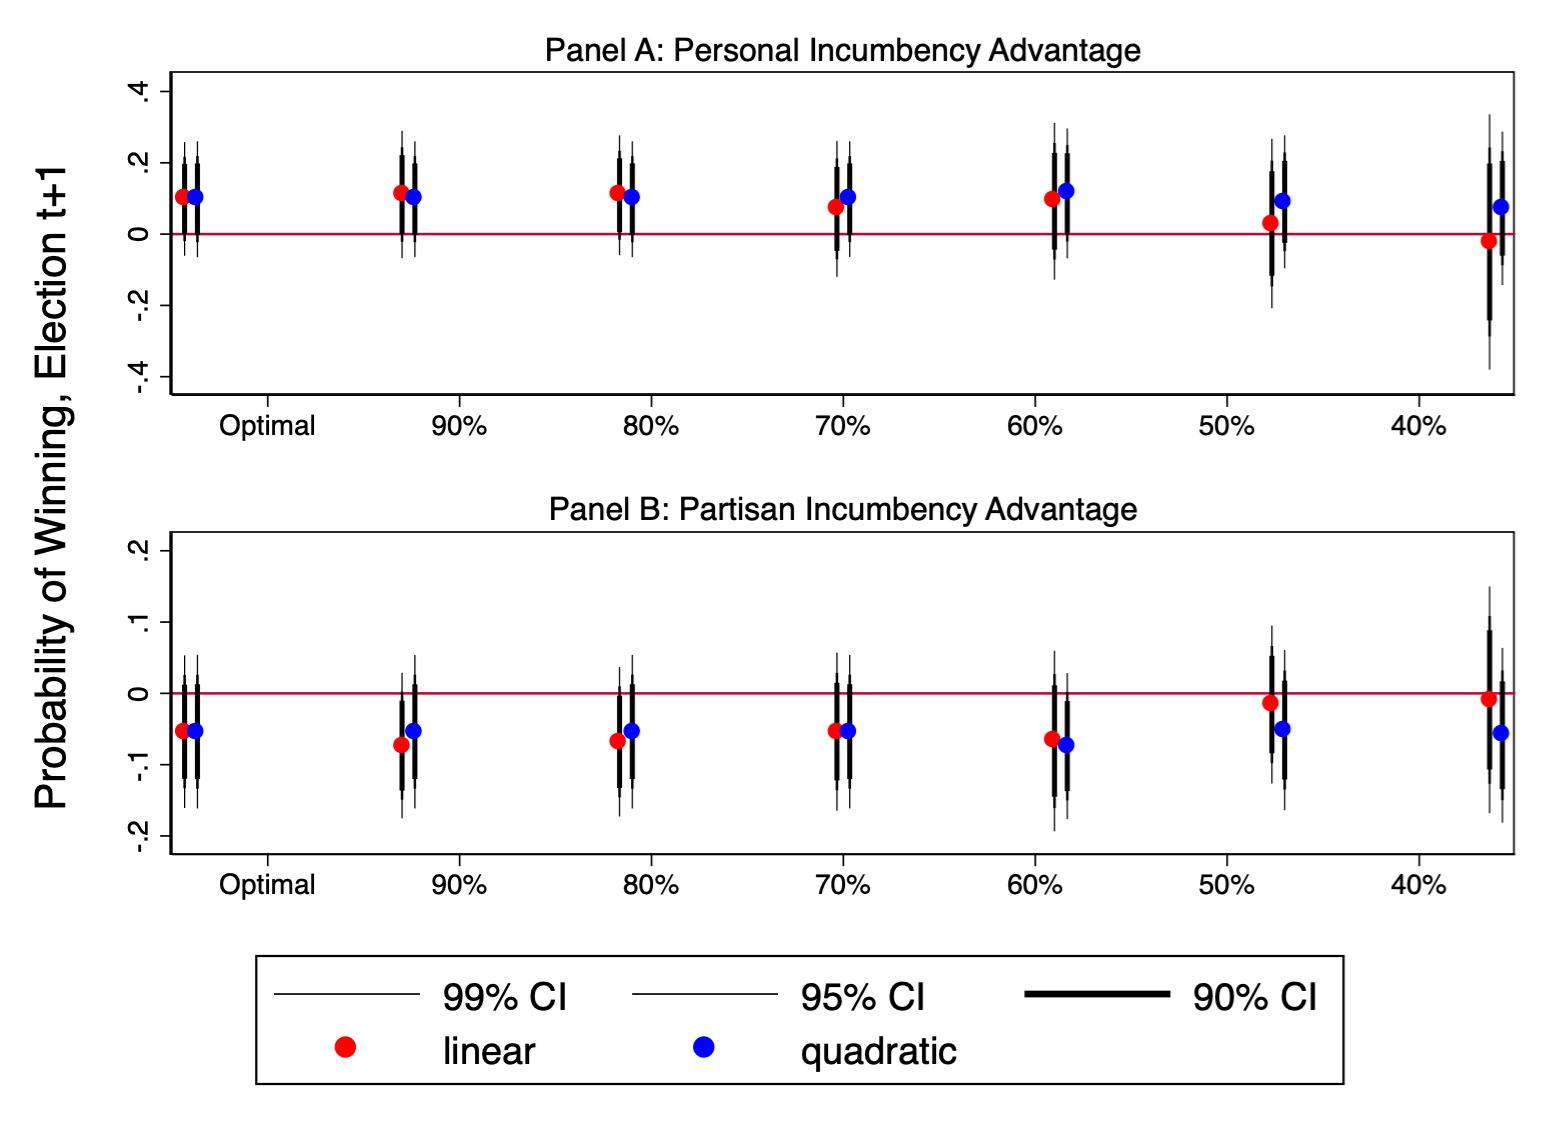
\includegraphics[width=0.65\textwidth]{Chapter2/Figures_incumbency/probability_bandwidths.png}
       \captionsetup{justification=centering}
 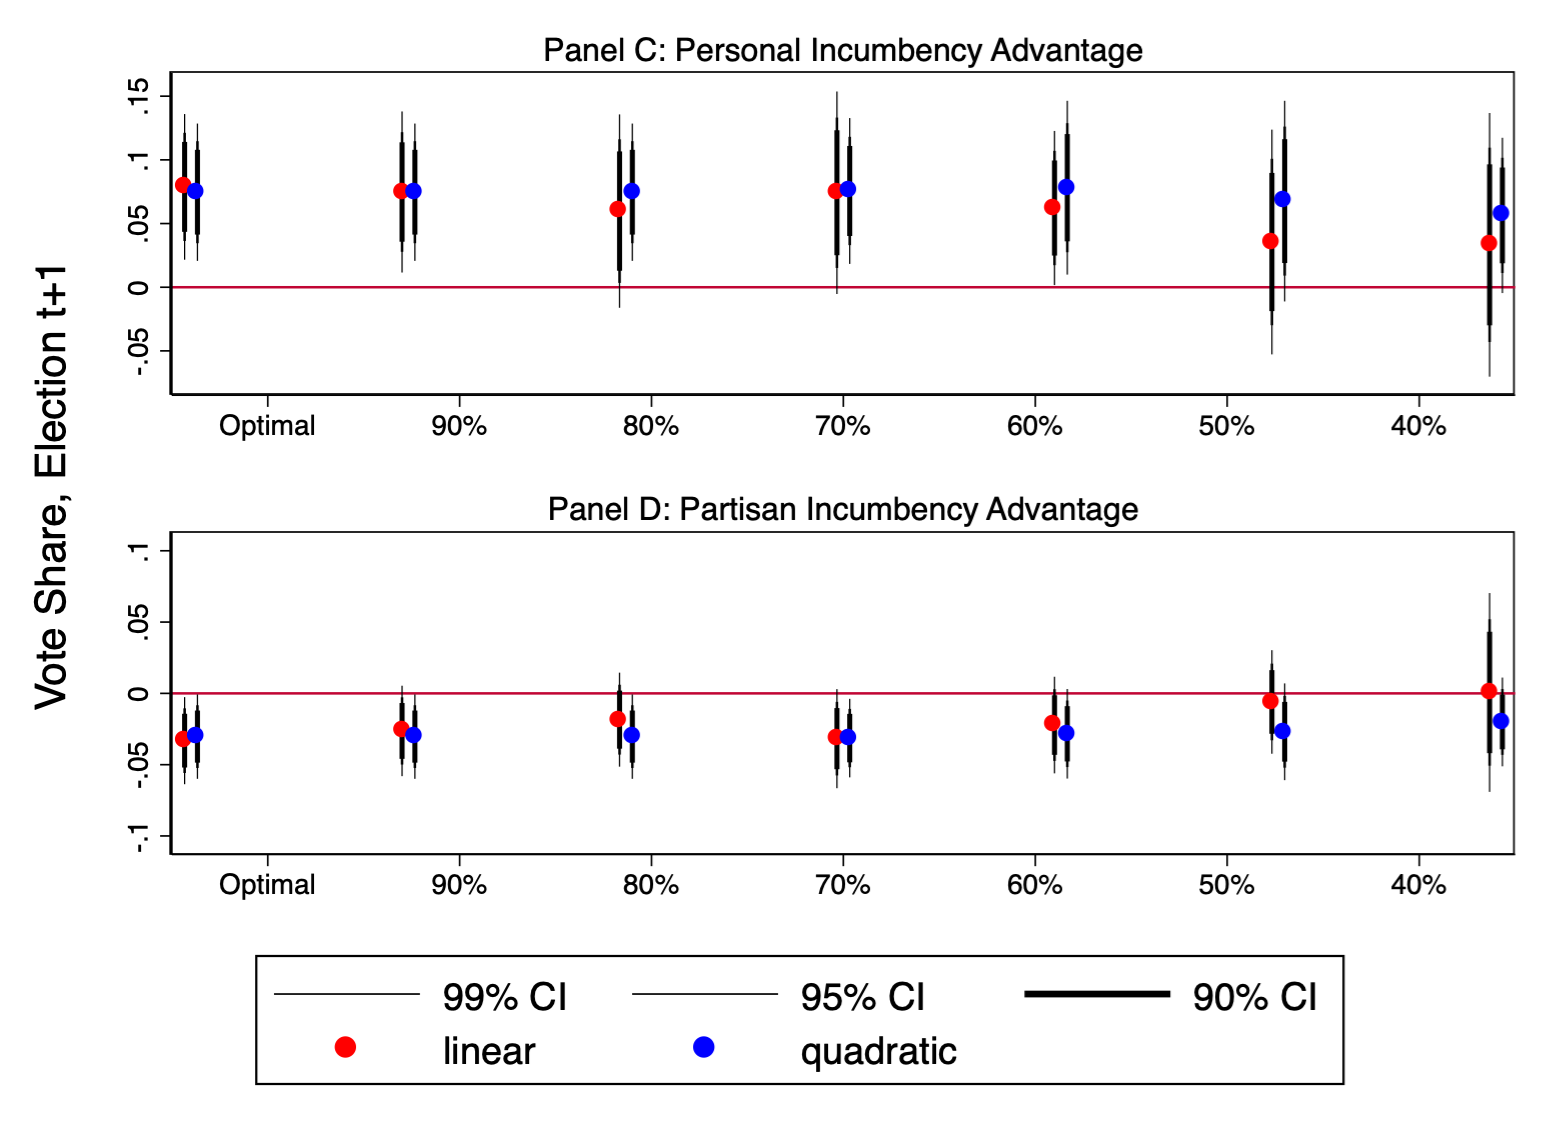
\includegraphics[width=0.65\textwidth]{Chapter2/Figures_incumbency/margin_bandwidths.png}

 \textbf{Note:} Figure \ref{fig:bandwidths} shows the average treatment effect of the Term Limit Reform on the probability of victory in the next election. Various bandwidths are tested as well as the optimal bandwidth following \citet{calonicoetal_2014}. A 90\% implies a reduction of the optimal bandwidth in 10\%, an 80\% a reduction of 20\%, and so on.
   
\end{figure} 
  